\documentclass[11pt]{article}

% ---------- Packages ----------
\usepackage[margin=0.75in]{geometry}
\usepackage{amsmath,amssymb,amsfonts}
\usepackage{mathtools}
\usepackage{array,booktabs,tabularx,multicol}
\usepackage{graphicx}
\usepackage{tikz,pgfplots}
\usepackage{tcolorbox}
\usepackage{xcolor}
\usepackage{enumitem}
\usepackage{fancyhdr}
\usepackage{lastpage}
\usepackage{needspace}

\pgfplotsset{compat=1.18}
\usetikzlibrary{arrows.meta,calc,angles,quotes,patterns}

% =========================
% Novel Prep Brand Colors
% =========================
\definecolor{nppurple}{RGB}{98,54,255}
\definecolor{nppurple2}{RGB}{76,42,204}
\definecolor{nplight}{RGB}{240,235,255}
\definecolor{npsoft}{RGB}{248,246,255}
\definecolor{npgray}{RGB}{226,222,238}

% ---------- Header/Footer ----------
\pagestyle{fancy}
\fancyhf{}
\lhead{\textcolor{nppurple2}{\textbf{Novel Prep Learning Center}}}
\rhead{\textcolor{nppurple2}{\textbf{Math II / Enhanced Math II Placement}}}
\cfoot{\textcolor{nppurple2}{\thepage\ of \pageref{LastPage}}}
\setlength{\headheight}{14pt}
\renewcommand{\headrulewidth}{0.4pt}
\renewcommand{\footrulewidth}{0pt}

% ---------- Boxes ----------
\newtcolorbox{titlebox}{
colback=nplight,
colframe=nppurple2,
boxrule=0.95pt,
arc=2pt,
left=8pt,
right=8pt,
top=8pt,
bottom=8pt
}

\newtcolorbox{problemBox}{
colback=white,
colframe=npgray,
boxrule=0.7pt,
arc=2pt,
left=8pt,
right=8pt,
top=8pt,
bottom=8pt
}

\newtcolorbox{scoreCard}{
colback=npsoft,
colframe=npgray,
boxrule=0.7pt,
arc=2pt,
left=8pt,
right=8pt,
top=8pt,
bottom=8pt
}

\newtcolorbox{sectionNote}{
colback=white,
colframe=nppurple2,
boxrule=0.75pt,
arc=2pt,
left=8pt,
right=8pt,
top=7pt,
bottom=7pt
}

\newtcolorbox{partBox}{
colback=nplight,
colframe=nppurple2,
boxrule=0.85pt,
arc=2pt,
left=8pt,
right=8pt,
top=6pt,
bottom=6pt
}

\setlength{\parindent}{0pt}
\setlength{\parskip}{0.35em}
\renewcommand{\arraystretch}{1.18}
\setlist[enumerate,1]{itemsep=0.75em,topsep=0.4em,label=\protect\circnum{\arabic*},leftmargin=*}
\setlist[enumerate,2]{itemsep=0.2em,topsep=0.2em}
\newcolumntype{L}[1]{>{\raggedright\arraybackslash}m{#1}}

% ---------- Commands ----------
\newcommand{\circnum}[1]{%
\begin{tikzpicture}[baseline=(char.base)]
\node[
draw=nppurple2,
circle,
inner sep=1.4pt,
line width=0.9pt,
text=nppurple2
] (char) {\strut\small #1};
\end{tikzpicture}}

\newcommand{\ansline}{\rule{2.5in}{0.4pt}}
\newcommand{\blankline}[1]{\rule{#1}{0.4pt}}
\newcommand{\work}{\vspace{1.8cm}}
\newcommand{\longwork}{\vspace{4.2cm}}

\newcommand{\grid}{
\begin{center}
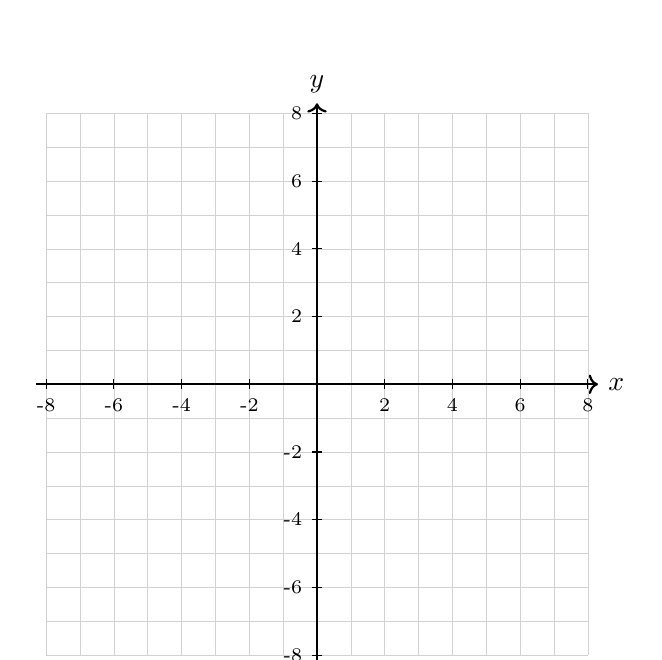
\begin{tikzpicture}[scale=0.43]
\draw[step=1cm,gray!35,very thin] (-8,-8) grid (8,8);
\draw[->,thick] (-8.3,0)--(8.3,0) node[right] {$x$};
\draw[->,thick] (0,-8.3)--(0,8.3) node[above] {$y$};
\foreach \x in {-8,-6,-4,-2,2,4,6,8} \draw (\x,0.15)--(\x,-0.15) node[below] {\scriptsize \x};
\foreach \y in {-8,-6,-4,-2,2,4,6,8} \draw (0.15,\y)--(-0.15,\y) node[left] {\scriptsize \y};
\end{tikzpicture}
\end{center}
}

\newcommand{\choices}[4]{
\begin{multicols}{4}
\begin{enumerate}[label=(\Alph*)]
\item #1
\item #2
\item #3
\item #4
\end{enumerate}
\end{multicols}
}

\newcommand{\choicesTwo}[4]{
\begin{multicols}{2}
\begin{enumerate}[label=(\Alph*)]
\item #1
\item #2
\item #3
\item #4
\end{enumerate}
\end{multicols}
}

\begin{document}

\begin{center}
    {\LARGE \textbf{Novel Prep Learning Center}}\\[0.2em]
    {\Large \textbf{Math II / Enhanced Math II Placement Exam}}\\[0.25em]
    {\large IUSD-Aligned Readiness Diagnostic}\\[0.6em]
    Name:\ \ansline \hfill Date:\ \ansline
\end{center}

\begin{titlebox}
\textbf{Directions:} Read each question carefully. Choose the best answer for multiple-choice questions. Show all work for graphing and free-response questions. Simplify exact answers when possible.
\end{titlebox}

\begin{problemBox}
\textbf{Teacher Use:} This diagnostic answers two placement questions. Gate 1 determines whether the student has enough readiness for Math II. Gate 2 should only be applied after Gate 1 is secure and determines whether the student is ready for Enhanced Math II.
\end{problemBox}

\begin{scoreCard}
\renewcommand{\arraystretch}{1.18}
\begin{tabularx}{\textwidth}{>{\bfseries\color{nppurple2}}L{2.7cm}X}
Scope & Quadratics, polynomial tools, radicals and rational exponents, complex numbers, probability, similarity, right-triangle trigonometry, circles, volume, statistics, conics, and advanced trigonometry.\\
Structure & 55 multiple-choice questions, 4 graphing/constructed-response questions, 10 free-response questions, scoring guide, study plan, and answer key.\\
Placement & Use Gate 1 first. Use Gate 2 only if the student's Math II readiness is already demonstrated.
\end{tabularx}
\end{scoreCard}

\newpage
\section*{Multiple Choice Questions}
\begin{sectionNote}
Questions 1-28 are used primarily for Math II readiness. Questions 29-55 add Enhanced Math II readiness signals, including Spring Final Review Units 6-11.
\end{sectionNote}

\begin{partBox}
{\large \textcolor{nppurple2}{\textbf{Part A --- Math II Readiness}}}
\end{partBox}

\begin{enumerate}
\item Which expression is equivalent to $\dfrac{a^3b^5}{a^{-1}b^2}$, assuming $a\neq 0$ and $b\neq 0$?
\choices{$a^2b^3$}{$a^4b^3$}{$a^3b^7$}{$\dfrac{b^3}{a^4}$}

\item Which expression shows the complete factorization of $9x^2+3x-2$?
\choices{$(3x+2)(3x-1)$}{$(9x-2)(x+1)$}{$(3x-2)(3x+1)$}{$(x+2)(9x-1)$}

\item The vertex of $y=(x-4)^2-7$ is:
\choices{$(-4,-7)$}{$(4,-7)$}{$(-4,7)$}{$(4,7)$}

\item What are the solutions of $x^2-5x-14=0$?
\choices{$x=2,-7$}{$x=7,-2$}{$x=-7,-2$}{$x=14,-1$}

\item The discriminant of $2x^2+4x+5=0$ indicates that the equation has:
\choices{two real rational solutions}{one real solution}{two real irrational solutions}{two non-real complex solutions}

\item Simplify $(3+2i)(4-i)$.
\choices{$10+5i$}{$14+5i$}{$14+11i$}{$12-2i$}

\item Evaluate $27^{2/3}$.
\choices{$3$}{$6$}{$9$}{$18$}

\item Simplify $\sqrt{75x^4}$, assuming $x$ is real.
\choices{$5x^2\sqrt{3}$}{$25x^2\sqrt{3}$}{$5x\sqrt{3}$}{$75x^2$}

\item Solve $\sqrt{x+5}=x-1$.
\choices{$x=1$}{$x=2$}{$x=4$}{No solution}

\item A quadratic function has zeros $-3$ and $5$ and opens upward. Which could be its equation?
\choices{$y=(x+3)(x-5)$}{$y=-(x+3)(x-5)$}{$y=(x-3)(x+5)$}{$y=-(x-3)(x+5)$}

\item What is the average rate of change of $f(x)=x^2-3x$ on the interval $[1,5]$?
\choices{$2$}{$3$}{$4$}{$8$}

\item Which table represents a quadratic function?
\begin{multicols}{2}
\begin{enumerate}[label=(\Alph*)]
\item $\begin{array}{c|cccc}x&0&1&2&3\\ \hline y&2&5&8&11\end{array}$
\item $\begin{array}{c|cccc}x&0&1&2&3\\ \hline y&1&3&7&13\end{array}$
\item $\begin{array}{c|cccc}x&0&1&2&3\\ \hline y&2&6&18&54\end{array}$
\item $\begin{array}{c|cccc}x&0&1&2&3\\ \hline y&4&4&4&4\end{array}$
\end{enumerate}
\end{multicols}

\item Simplify $(2x^2-3x+4)+(x^2+5x-7)$.
\choices{$3x^2+2x-3$}{$3x^2-8x+11$}{$2x^4-15x^2-28$}{$x^2+2x-3$}

\item Expand $(x-4)(x+6)$.
\choices{$x^2+2x-24$}{$x^2-2x-24$}{$x^2+10x-24$}{$x^2+2x+24$}

\item A class has 18 students who play a sport, 12 students who do not, and 10 of the athletes are girls. If one student is selected from the class, what is $P(\text{athlete})$?
\choices{$\frac{3}{5}$}{$\frac{2}{5}$}{$\frac{1}{3}$}{$\frac{5}{9}$}

\item If $P(A)=0.62$, what is $P(A^c)$?
\choices{$0.38$}{$0.62$}{$1.62$}{$-0.38$}

\item If events $A$ and $B$ are independent with $P(A)=0.4$ and $P(B)=0.7$, then $P(A\text{ and }B)$ is:
\choices{$0.11$}{$0.28$}{$0.30$}{$1.10$}

\item How many ways can a committee of 3 students be chosen from 8 students?
\choices{$24$}{$56$}{$336$}{$512$}

\item A dilation centered at the origin with scale factor $3$ maps $(2,-5)$ to:
\choices{$(5,-2)$}{$(6,-15)$}{$(-6,15)$}{$(\frac{2}{3},-\frac{5}{3})$}

\item If two triangles are similar with scale factor $2$ from the smaller triangle to the larger triangle, then the ratio of their areas is:
\choices{$1:2$}{$1:4$}{$2:1$}{$4:1$}

\item In a right triangle, an acute angle $\theta$ has opposite side $7$ and hypotenuse $25$. What is $\sin\theta$?
\choices{$\frac{7}{25}$}{$\frac{24}{25}$}{$\frac{7}{24}$}{$\frac{24}{7}$}

\item A $30^\circ$-$60^\circ$-$90^\circ$ triangle has short leg $6$. What is the hypotenuse?
\choices{$6\sqrt{3}$}{$12$}{$3\sqrt{3}$}{$18$}

\item The equation of a circle with center $(2,-3)$ and radius $5$ is:
\choicesTwo{$(x-2)^2+(y+3)^2=25$}{$(x+2)^2+(y-3)^2=25$}{$(x-2)^2+(y+3)^2=5$}{$(x+2)^2+(y-3)^2=5$}

\item In a circle, an inscribed angle intercepts an arc measuring $110^\circ$. What is the measure of the inscribed angle?
\choices{$55^\circ$}{$70^\circ$}{$110^\circ$}{$220^\circ$}

\item A cylinder has radius $3$ and height $10$. What is its volume?
\choices{$30\pi$}{$60\pi$}{$90\pi$}{$300\pi$}

\item Which equation represents a parabola with vertex $(1,-4)$ that opens upward?
\choices{$y=(x-1)^2-4$}{$y=(x+1)^2-4$}{$y=-(x-1)^2-4$}{$y=(x-1)^2+4$}

\item Solve $x^2= -49$.
\choices{$x=7$}{$x=-7$}{$x=\pm 7i$}{No solution}

\item Which statement best describes the graph of $y=|x+2|-3$?
\choicesTwo{Vertex $(-2,-3)$ and opens upward}{Vertex $(2,-3)$ and opens upward}{Vertex $(-2,3)$ and opens downward}{Vertex $(2,3)$ and opens downward}

\newpage
\begin{partBox}
{\large \textcolor{nppurple2}{\textbf{Part B --- Enhanced Math II Readiness}}}
\end{partBox}

\item Which piecewise function equals $2x+1$ for $x<0$ and $x^2$ for $x\geq 0$?
\choicesTwo{$f(x)=\begin{cases}x^2,&x<0\\2x+1,&x\geq0\end{cases}$}{$f(x)=\begin{cases}2x+1,&x<0\\x^2,&x\geq0\end{cases}$}{$f(x)=|2x+1|$}{$f(x)=x^2+2x+1$}

\item The standard deviation of a data set measures:
\choicesTwo{the center of the data}{the spread of the data from the mean}{the largest value}{the middle value}

\item A score is $84$ on a normal distribution with mean $72$ and standard deviation $6$. What is the $z$-score?
\choices{$-2$}{$-1$}{$1$}{$2$}

\item For a normal distribution, approximately what percent of data falls within one standard deviation of the mean?
\choices{$34\%$}{$68\%$}{$95\%$}{$99.7\%$}

\item A confidence interval for a population proportion is $(0.41,0.53)$. Its point estimate is:
\choices{$0.06$}{$0.12$}{$0.47$}{$0.94$}

\item Which equation represents an ellipse centered at the origin with horizontal major axis length $10$ and vertical minor axis length $6$?
\choicesTwo{$\frac{x^2}{25}+\frac{y^2}{9}=1$}{$\frac{x^2}{9}+\frac{y^2}{25}=1$}{$\frac{x^2}{10}+\frac{y^2}{6}=1$}{$\frac{x^2}{5}+\frac{y^2}{3}=1$}

\item A parabola has vertex $(2,-1)$ and directrix $y=-3$. Which equation represents the parabola?
\choicesTwo{$(x-2)^2=8(y+1)$}{$(x-2)^2=-8(y+1)$}{$(y+1)^2=8(x-2)$}{$(y+1)^2=-8(x-2)$}

\item Convert $150^\circ$ to radians.
\choices{$\frac{5\pi}{6}$}{$\frac{2\pi}{3}$}{$\frac{3\pi}{4}$}{$\frac{7\pi}{6}$}

\Needspace{6\baselineskip}
\item Evaluate $\sin\left(\frac{3\pi}{2}\right)$.
\choices{$-1$}{$0$}{$1$}{$\frac{\sqrt{2}}{2}$}

\Needspace{6\baselineskip}
\item Evaluate $\tan(210^\circ)$.
\choices{$-\sqrt{3}$}{$-\frac{\sqrt{3}}{3}$}{$\frac{\sqrt{3}}{3}$}{$\sqrt{3}$}

\item A triangle has sides $a=7$, $b=10$, and included angle $C=60^\circ$. By the Law of Cosines, $c^2$ equals:
\choices{$49$}{$79$}{$149$}{$249$}

\item In $\triangle ABC$, $A=35^\circ$, $a=8$, and $b=10$. Which law would be used first to determine possible measures of angle $B$?
\choices{Pythagorean Theorem}{Law of Sines}{Law of Cosines}{Area formula}

\item A sector has radius $6$ and central angle $\frac{2\pi}{3}$ radians. What is its arc length?
\choices{$4\pi$}{$6\pi$}{$12\pi$}{$24\pi$}

\item A chord of a circle is perpendicular to a radius. What must be true?
\choices{The radius bisects the chord}{The chord is a diameter}{The chord is tangent}{The radius is twice the chord}

\item If two tangents are drawn from the same external point to a circle, then:
\choices{the tangent segments are congruent}{the tangents are parallel}{the intercepted arcs are equal to $90^\circ$}{the tangents pass through the center}

\item A hyperbola has center $(0,0)$, vertices $(\pm 4,0)$, and foci $(\pm 5,0)$. Which equation represents it?
\choices{$\frac{x^2}{16}-\frac{y^2}{9}=1$}{$\frac{y^2}{16}-\frac{x^2}{9}=1$}{$\frac{x^2}{9}-\frac{y^2}{16}=1$}{$\frac{x^2}{25}-\frac{y^2}{16}=1$}

\item A cone has radius $4$ and height $9$. What is its volume?
\choices{$12\pi$}{$36\pi$}{$48\pi$}{$144\pi$}

\newpage
\item The table shows activity choices.
\[
\begin{array}{|c|c|c|c|}
\hline
&\text{STEM Club}&\text{Arts Club}&\text{Total}\\ \hline
\text{Grade 9}&18&12&30\\ \hline
\text{Grade 10}&10&20&30\\ \hline
\text{Total}&28&32&60\\ \hline
\end{array}
\]
What is $P(\text{Arts Club}\mid \text{Grade 10})$?
\choices{$\frac{1}{3}$}{$\frac{2}{3}$}{$\frac{1}{2}$}{$\frac{5}{8}$}

\item A club has 9 students. How many ways can it choose a president, vice president, and secretary if no student can hold more than one position?
\choices{$84$}{$504$}{$729$}{$362{,}880$}

\item A histogram is strongly skewed right. Which statement is usually true?
\choicesTwo{The mean is greater than the median.}{The mean is less than the median.}{The mean equals the median.}{The standard deviation must be $0$.}

\item Two triangles have two pairs of corresponding angles congruent. Which similarity criterion proves the triangles similar?
\choices{SSS similarity}{SAS similarity}{AA similarity}{HL congruence}

\item The measure of one interior angle of a parallelogram is $30^\circ$ less than 9 times the measure of another angle. What is the smaller angle?
\choices{$21^\circ$}{$30^\circ$}{$80^\circ$}{$159^\circ$}

\item In $\triangle ABC$, $A=35^\circ$, $a=12$, and $b=18$. Which statement is true?
\choicesTwo{There is no possible triangle.}{There is exactly one possible triangle.}{The triangle must be right.}{There are two possible triangles.}

\item Convert $\frac{7\pi}{12}$ radians to degrees.
\choices{$90^\circ$}{$100^\circ$}{$105^\circ$}{$120^\circ$}

\item Two chords intersect inside a circle. One chord has segments $6$ and $8$; the other has segments $x$ and $12$. Find $x$.
\choices{$4$}{$6$}{$9$}{$16$}

\Needspace{6\baselineskip}
\item A sector has radius $5$ and central angle $\frac{4\pi}{5}$ radians. What is the area of the sector?
\choices{$5\pi$}{$10\pi$}{$20\pi$}{$25\pi$}

\item Two tangents from an external point intercept a major arc of $220^\circ$ and a minor arc of $140^\circ$. What is the measure of the angle formed by the tangents?
\choices{$40^\circ$}{$70^\circ$}{$80^\circ$}{$180^\circ$}
\end{enumerate}

\newpage
\section*{Graphing and Constructed Response}
\begin{partBox}
{\large \textcolor{nppurple2}{\textbf{Part C --- Graphs, Models, and Diagrams}}}
\end{partBox}

\begin{enumerate}
\item Graph $y=(x-1)^2-4$. Label the vertex and the $x$-intercepts.
\grid

\newpage
\item Graph the piecewise function.
\[
f(x)=
\begin{cases}
x+2, & x<1,\\
-2x+5, & x\geq 1.
\end{cases}
\]
\grid

\newpage
\item In the diagram, lines $\ell$ and $m$ are parallel. Find $x$ and justify your answer.
\begin{center}
\begin{tikzpicture}[scale=0.9]
\draw[thick] (-4,1.5)--(4,1.5) node[right] {$\ell$};
\draw[thick] (-4,-1.5)--(4,-1.5) node[right] {$m$};
\draw[thick] (-2.5,-2.3)--(2.6,2.3);
\node at (-0.15,1.9) {$112^\circ$};
\node at (-2.25,-1.1) {$(3x+7)^\circ$};
\draw[->] (-4.2,1.5)--(-3.8,1.5);
\draw[->] (-4.2,-1.5)--(-3.8,-1.5);
\end{tikzpicture}
\end{center}
\longwork

\newpage
\item In circle $O$, $PT$ and $PS$ are tangent segments from the same external point $P$. If $PT=3x+5$ and $PS=5x-9$, find $x$ and each tangent length.
\begin{center}
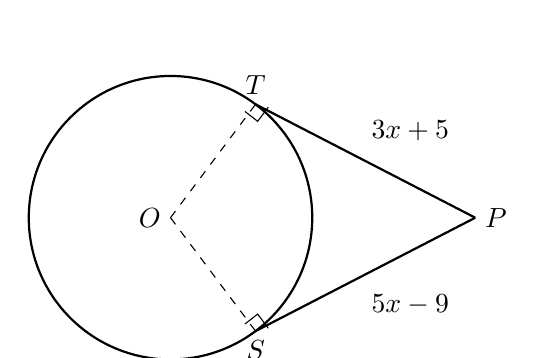
\begin{tikzpicture}[scale=0.9]
\coordinate (O) at (0,0);
\coordinate (T) at (1.2,1.6);
\coordinate (S) at (1.2,-1.6);
\coordinate (P) at (4.3,0);
\draw[thick] (O) circle (2);
\draw[thick] (P)--(T);
\draw[thick] (P)--(S);
\draw[dashed] (O)--(T);
\draw[dashed] (O)--(S);
\node[left] at (O) {$O$};
\node[above] at (T) {$T$};
\node[below] at (S) {$S$};
\node[right] at (P) {$P$};
\node[above right] at (2.7,0.95) {$3x+5$};
\node[below right] at (2.7,-0.95) {$5x-9$};
\draw (T)++(-0.15,-0.1)--++(0.18,-0.14)--++(0.15,0.2);
\draw (S)++(-0.15,0.1)--++(0.18,0.14)--++(0.15,-0.2);
\end{tikzpicture}
\end{center}
\longwork
\end{enumerate}

\newpage
\section*{Free Response Questions}
\begin{partBox}
{\large \textcolor{nppurple2}{\textbf{Part D --- Placement Reasoning Tasks}}}
\end{partBox}

\begin{enumerate}
\item \textbf{Quadratic Modeling.} A ball is launched from a platform. Its height in feet after $t$ seconds is modeled by
\[
h(t)=-16t^2+64t+80.
\]
\begin{enumerate}[label=(\alph*)]
\item Find the maximum height and the time when it occurs.
\item Find when the ball hits the ground.
\item Explain what the $h$-intercept means in context.
\end{enumerate}
\longwork

\item \textbf{Polynomial and Complex Number Fluency.} 
\begin{enumerate}[label=(\alph*)]
\item Factor $2x^2-7x-15$ completely.
\item Solve $2x^2-7x-15=0$.
\item Simplify $(5-3i)-(2+4i)$.
\end{enumerate}
\longwork

\newpage
\item \textbf{Radicals and Rational Exponents.}
\begin{enumerate}[label=(\alph*)]
\item Simplify $\sqrt{108x^6}$ assuming $x$ is real.
\item Rewrite $\sqrt[3]{x^5}$ using rational exponents.
\item Solve $\sqrt{x+3}=x+1$ and check for extraneous solutions.
\end{enumerate}
\longwork

\item \textbf{Probability.} A bag contains 5 red, 4 blue, and 3 green tiles. Two tiles are drawn without replacement.
\begin{enumerate}[label=(\alph*)]
\item Find the probability both tiles are blue.
\item Find the probability the first tile is red and the second tile is green.
\item Find the probability at least one of the two tiles is green.
\end{enumerate}
\longwork

\newpage
\item \textbf{Similarity and Trigonometry.} A person standing 48 feet from a building measures an angle of elevation of $38^\circ$ to the top of the building. The person's eye height is 5 feet.
\begin{enumerate}[label=(\alph*)]
\item Draw and label a right-triangle model.
\item Find the height of the building to the nearest foot.
\item State which trigonometric ratio you used and why.
\end{enumerate}
\longwork

\item \textbf{Enhanced Statistics.} A normally distributed test has mean $76$ and standard deviation $8$.
\begin{enumerate}[label=(\alph*)]
\item Find the $z$-score for a score of $92$.
\item Approximate the percentile for a score of $92$ using the empirical rule.
\item A student scored $68$. Explain whether $92$ or $68$ is more unusual.
\end{enumerate}
\longwork

\newpage
\item \textbf{Enhanced Conics.}
\begin{enumerate}[label=(\alph*)]
\item Write the equation of the circle with center $(-3,4)$ and circumference $10\pi$.
\item Write the equation of the ellipse centered at $(1,-2)$ with horizontal semi-major axis $5$ and vertical semi-minor axis $3$.
\item Write the equation of the parabola with vertex $(0,1)$ and directrix $y=-1$.
\end{enumerate}
\longwork

\item \textbf{Enhanced Triangle Trigonometry.} In $\triangle ABC$, $a=12$, $b=15$, and $C=42^\circ$.
\begin{enumerate}[label=(\alph*)]
\item Use the Law of Cosines to find side $c$ to the nearest tenth.
\item Find the area of the triangle to the nearest tenth.
\item Explain why right-triangle trigonometry alone is not enough for this triangle.
\end{enumerate}
\longwork

\newpage
\item \textbf{Law of Sines and the Ambiguous Case.} In $\triangle ABC$, $A=35^\circ$, $a=12$, and $b=18$.
\begin{enumerate}[label=(\alph*)]
\item Use the Law of Sines to find all possible measures of angle $B$ to the nearest tenth.
\item Find the corresponding possible measures of angle $C$.
\item Explain why this information creates the ambiguous case.
\end{enumerate}
\longwork

\item \textbf{Circle Relationships and Sector Area.}
\begin{enumerate}[label=(\alph*)]
\item Two chords intersect inside a circle. One chord has segments $5$ and $12$; the other has segments $6$ and $x$. Find $x$.
\item A circle has radius $6$. A sector has area $15\pi$. Find the central angle in radians.
\item Find the arc length of that sector.
\end{enumerate}
\longwork
\end{enumerate}

\newpage
\section*{Teacher Scoring Guide}
\begin{titlebox}
\textbf{Suggested point values:} Multiple Choice 55 points; Graphing/Constructed Response 16 points; Free Response 60 points. Total: 131 points.
\end{titlebox}

\begin{problemBox}
\textbf{IUSD alignment used for this diagnostic:}
\begin{itemize}
\item \textbf{Math II:} quadratic and absolute value functions, polynomial expressions, quadratic equations with complex numbers, rational exponents and radicals, probability, similarity and proof, right-triangle trigonometry, circles, volume, and algebra/geometry modeling.
\item \textbf{Enhanced Math II:} all Math II expectations, plus piecewise functions, stronger polynomial tools, statistics including normal distributions and standard deviation, conics, advanced triangle trigonometry, unit circle/radian fluency, and deeper circle relationships.
\end{itemize}
\end{problemBox}

\begin{sectionNote}
\textbf{Two-Gate Placement Protocol}
\end{sectionNote}
\begin{center}
\renewcommand{\arraystretch}{1.25}
\begin{tabular}{|L{3.0cm}|L{4.4cm}|L{6.2cm}|}
\hline
\textbf{Decision Gate} & \textbf{Use These Items} & \textbf{Decision Rule}\\
\hline
Gate 1: Math II qualification & MC 1-28, Graphing 1 and 3, FR 1-5. Maximum 66 points. & 
50-66: qualified for Math II. 43-49: borderline; Math II with support. Below 43: not ready for Math II without remediation.\\
\hline
Gate 2: Enhanced Math II qualification & Only apply if Gate 1 is passed. Use MC 29-55, Graphing 2 and 4, FR 6-10. Maximum 65 points. &
50-65 and MC Part B at least 21/27: qualified for Enhanced Math II. 43-49: borderline Enhanced; targeted preparation recommended. Below 43: place in Math II or build first.\\
\hline
\end{tabular}
\end{center}

\begin{titlebox}
\textbf{Important placement note:} A student should not be placed into Enhanced Math II if the student is weak on quadratics, polynomial operations, radicals, probability, and similarity, even if the student has seen some later topics such as conics or trigonometry.
\end{titlebox}

\newpage
\section*{Study Plan by Diagnostic Band}
\begin{sectionNote}
\textbf{Lesson length assumption:} one lesson is 90 minutes. If lessons are 60 minutes, multiply the lesson count by about 1.5.
\end{sectionNote}

\begin{center}
\renewcommand{\arraystretch}{1.25}
\begin{tabular}{|L{3.0cm}|L{3.8cm}|L{6.6cm}|}
\hline
\textbf{Band} & \textbf{Recommended Lessons} & \textbf{Focus}\\
\hline
Below Math II readiness & 24-32 lessons & Algebra I recovery, factoring, solving equations, function notation, graphing, exponent rules, radicals, and core geometry vocabulary. Goal: pass Gate 1 reliably.\\
\hline
Borderline Math II & 14-20 lessons & Quadratic representations, factoring and completing the square, complex numbers, radicals, basic probability, similarity, and right-triangle trigonometry.\\
\hline
Math II ready, not Enhanced ready & 18-26 lessons & Piecewise functions, statistics, normal models, conics, unit circle values, Law of Sines/Cosines, circle theorems, and multi-step modeling.\\
\hline
Borderline Enhanced & 8-12 lessons & Enhanced-level mixed review: advanced trig, conics, statistics interpretation, circle proof/arc relationships, and explanation quality.\\
\hline
Enhanced ready & 4-6 lessons & Maintenance and enrichment: proof writing, non-routine modeling, conic/trig fluency, and accuracy under timed conditions.\\
\hline
\end{tabular}
\end{center}

\newpage
\begin{sectionNote}
\textbf{Module Map}
\end{sectionNote}
\begin{center}
\renewcommand{\arraystretch}{1.25}
\begin{tabular}{|L{4.0cm}|L{2.1cm}|L{7.0cm}|}
\hline
\textbf{Module} & \textbf{Lessons} & \textbf{When to assign}\\
\hline
Quadratic foundations & 4-6 & Misses MC 2-5, 10-12, 26, 28, FR1.\\
\hline
Polynomial tools and complex numbers & 4-6 & Misses MC 1, 6, 13-14, 27, FR2.\\
\hline
Radicals and rational exponents & 3-5 & Misses MC 7-9, FR3.\\
\hline
Probability and counting & 3-5 & Misses MC 15-18, 46-47, FR4.\\
\hline
Similarity, proof, and geometry & 5-7 & Misses MC 19-20, 23-25, 49-50, Graphing 3-4, FR5.\\
\hline
Enhanced statistics & 3-5 & Misses MC 30-33, FR6.\\
\hline
Conics and circle equations & 4-6 & Misses MC 34-36, 43, FR7.\\
\hline
Advanced trigonometry & 4-6 & Misses MC 37-42, 51-52, FR8-9.\\
\hline
Circle relationships and sector geometry & 3-5 & Misses MC 42-43, 53-55, Graphing 4, FR10.\\
\hline
\end{tabular}
\end{center}

\newpage
\section*{Answer Key and Selected Free Response Answers}
\begin{sectionNote}
Use this page for quick grading. Selected free-response answers show essential results; full credit should still depend on clear work and reasoning.
\end{sectionNote}

\textbf{Multiple Choice Answer Key}
\begin{center}
\renewcommand{\arraystretch}{1.2}
\begin{tabular}{|c|ccccccccc|}
\hline
Q & 1&2&3&4&5&6&7&8&9\\ \hline
Ans & B&A&B&B&D&B&C&A&C\\ \hline
\end{tabular}

\begin{tabular}{|c|ccccccccc|}
\hline
Q & 10&11&12&13&14&15&16&17&18\\ \hline
Ans & A&B&B&A&A&A&A&B&B\\ \hline
\end{tabular}

\begin{tabular}{|c|ccccccccc|}
\hline
Q & 19&20&21&22&23&24&25&26&27\\ \hline
Ans & B&B&A&B&A&A&C&A&C\\ \hline
\end{tabular}

\begin{tabular}{|c|ccccccccc|}
\hline
Q & 28&29&30&31&32&33&34&35&36\\ \hline
Ans & A&B&B&D&B&C&A&A&A\\ \hline
\end{tabular}

\begin{tabular}{|c|ccccccccc|}
\hline
Q & 37&38&39&40&41&42&43&44&45\\ \hline
Ans & A&C&B&B&A&A&A&A&C\\ \hline
\end{tabular}

\begin{tabular}{|c|cccccccccc|}
\hline
Q & 46&47&48&49&50&51&52&53&54&55\\ \hline
Ans & B&B&A&C&A&D&C&A&B&A\\ \hline
\end{tabular}
\end{center}

\textbf{Constructed Response Answers}
\begin{itemize}
\item G1: Vertex $(1,-4)$; $x$-intercepts $(-1,0)$ and $(3,0)$.
\item G2: Line $y=x+2$ for $x<1$ with open point at $(1,3)$; line $y=-2x+5$ for $x\geq1$ with closed point at $(1,3)$.
\item G3: $3x+7=112$, so $x=35$ using corresponding angles.
\item G4: $3x+5=5x-9$, so $x=7$ and each tangent length is $26$.
\end{itemize}

\textbf{Selected Free Response Answers}
\begin{itemize}
\item FR1: Vertex time $t=2$; maximum height $144$ ft; hits ground at $t=5$ sec; $h(0)=80$ is initial height.
\item FR2: $(2x+3)(x-5)$; $x=-\frac{3}{2},5$; $3-7i$.
\item FR3: $6|x^3|\sqrt{3}$; $x^{5/3}$; solution $x=1$ only.
\item FR4: $\frac{1}{11}$; $\frac{5}{44}$; $\frac{5}{11}$.
\item FR5: Height $\approx 48\tan(38^\circ)+5\approx 43$ ft; tangent is used because opposite and adjacent sides are involved.
\item FR6: $z=2$; about 97.5th percentile; both $92$ and $68$ are 2 standard deviations from the mean, so equally unusual by distance.
\item FR7: $(x+3)^2+(y-4)^2=25$; $\frac{(x-1)^2}{25}+\frac{(y+2)^2}{9}=1$; $x^2=8(y-1)$.
\item FR8: $c\approx10.0$; area $\approx60.2$ square units; the triangle is not given as right, so Law of Cosines/area with included angle is needed.
\item FR9: $\sin B=\frac{18\sin35^\circ}{12}$, so $B\approx59.4^\circ$ or $120.6^\circ$; $C\approx85.6^\circ$ or $24.4^\circ$.
\item FR10: $x=10$; central angle $\theta=\frac{5\pi}{6}$; arc length $5\pi$.
\end{itemize}

\end{document}
